\subsection{Montaje del prototipo}

Para hacer el montaje del sistema en el prototipado, se ha utilizado una placa de madera de contrachapado para poder atornillar los componentes y que queden fijos. Se ha podido aprovechar que casi todas las placas de los módulos cuentan con perforaciones que hemos podido utilizar para colocar tornillos. 

Las conexiones entre cables, para asegurar su firmeza y seguridad sin comprometer la rápida conexión y modificación del circuito, han sido realizadas con regletas de clemas y con conectores de conexión rápida. Por otro lado, las conexiones con algunos módulos se han podido realizar con terminales de tornillo. Por último, hemos utilizado abrazaderas de clavo para guiar los cables y fijar las dos placas que no tienen agujeros. Todos estos conectores se pueden ver en la \autoref{fig:hardware/proto/conectores}.
\begin{figure}[H]
    \centering
    \begin{subfigure}[b]{0.25\textwidth}
        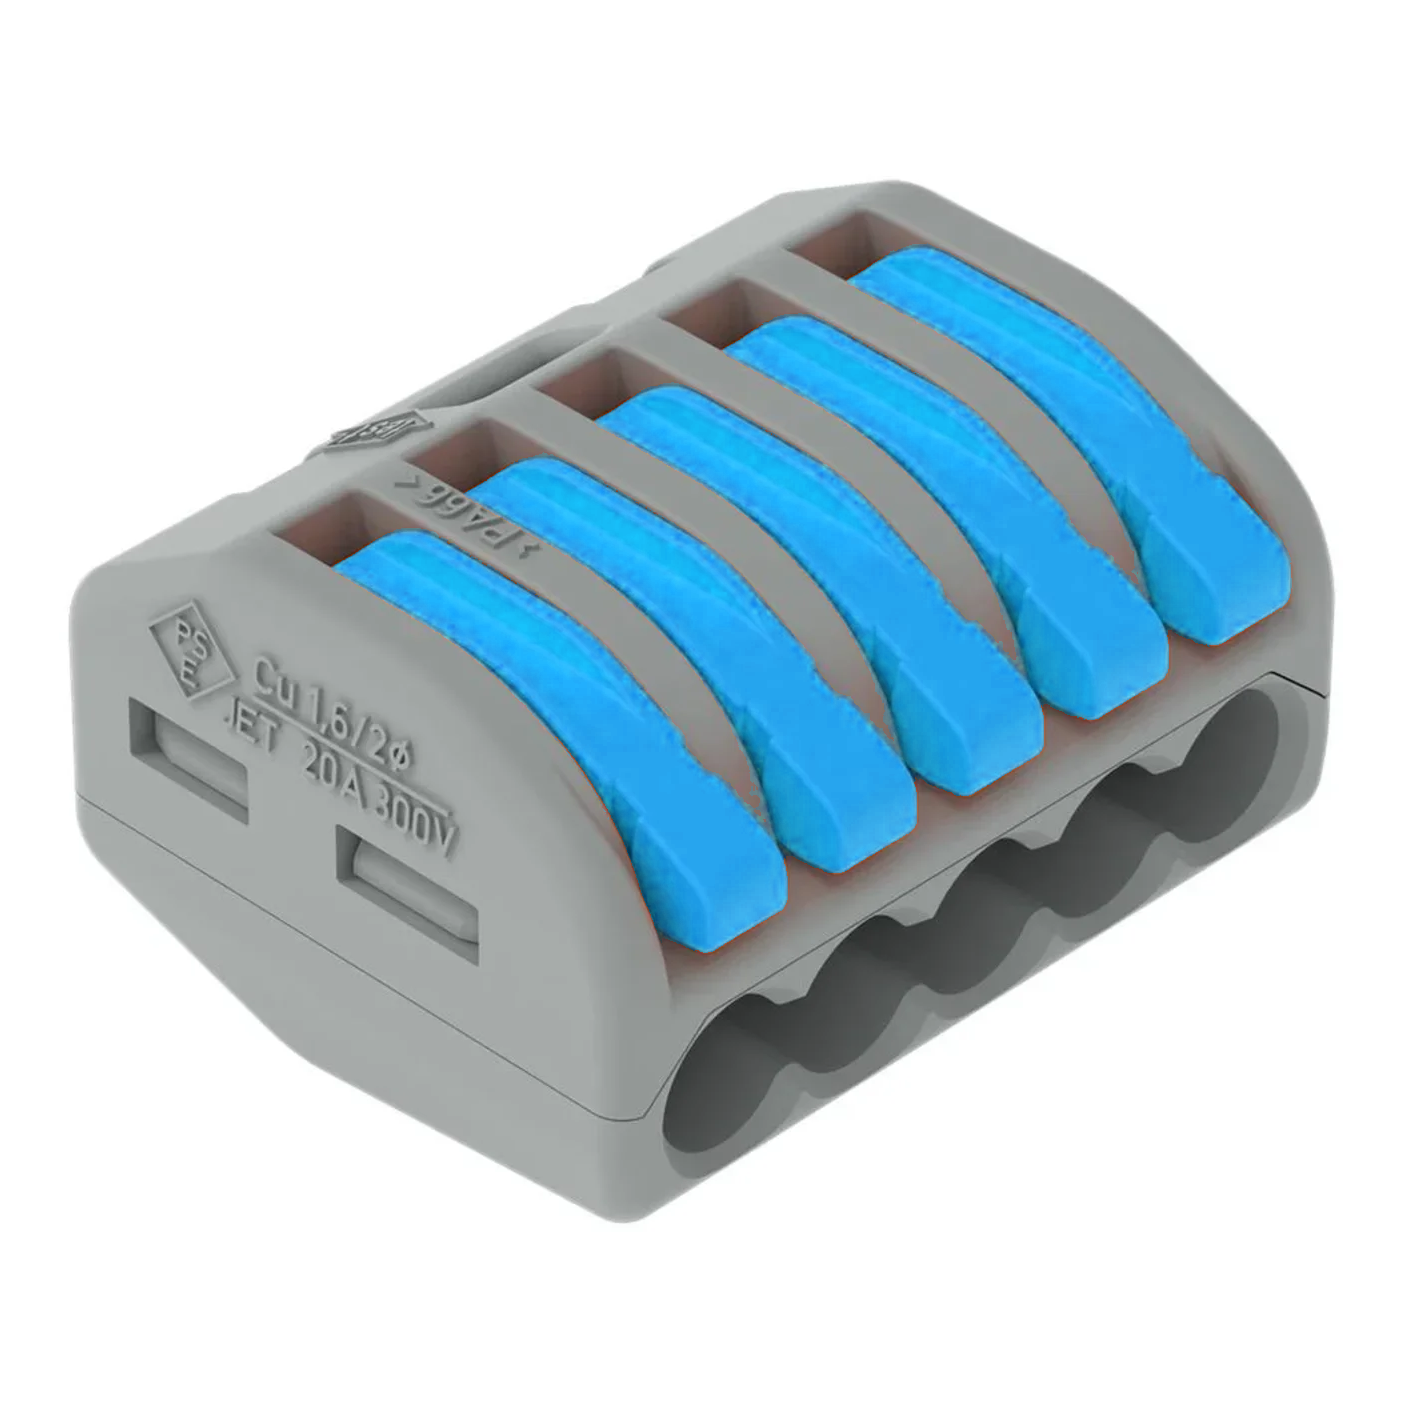
\includegraphics[width=\textwidth]{images/2-hardware/wago.png}       
        \caption{Conexión rápida}
    \end{subfigure}
    \hspace{2cm}
    \begin{subfigure}[b]{0.25\textwidth}
        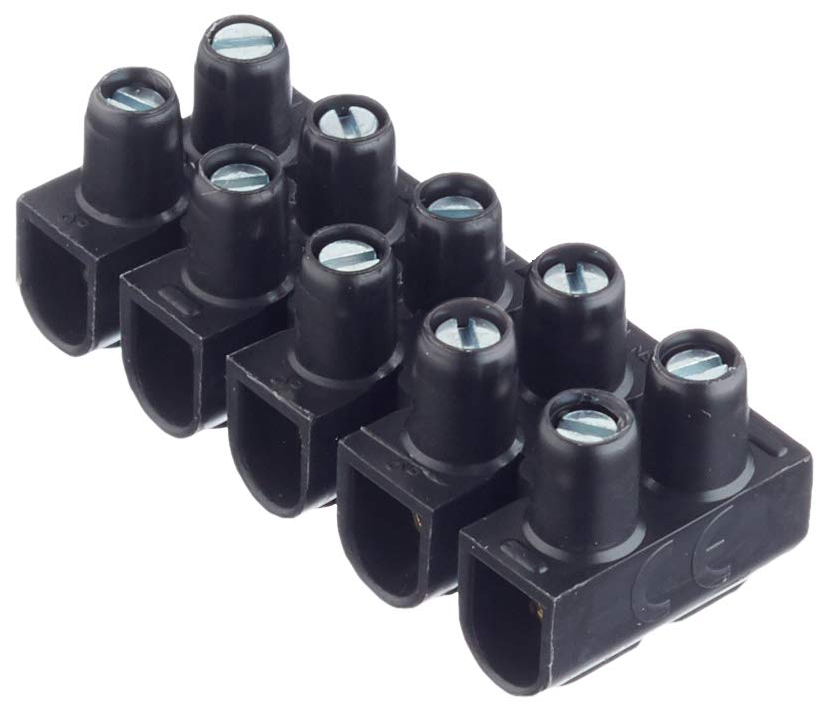
\includegraphics[width=\textwidth]{images/2-hardware/regletas.png}
        \caption{Regletas de clemas}
    \end{subfigure}
    \\
    \begin{subfigure}[b]{0.25\textwidth}
        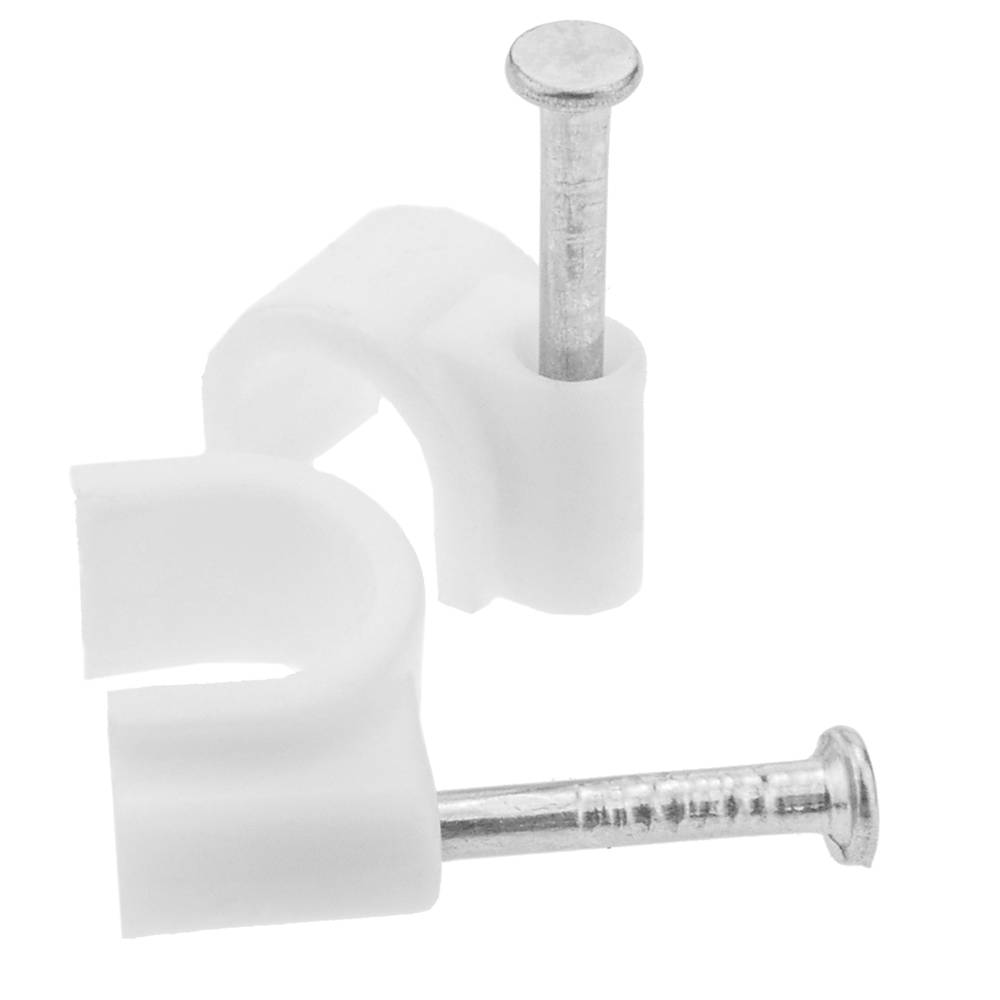
\includegraphics[width=\textwidth]{images/2-hardware/abrazaderaClavo.png}
        \caption{Abrazaderas de clavo}
    \end{subfigure}
    \hspace{2cm}
    \begin{subfigure}[b]{0.25\textwidth}
        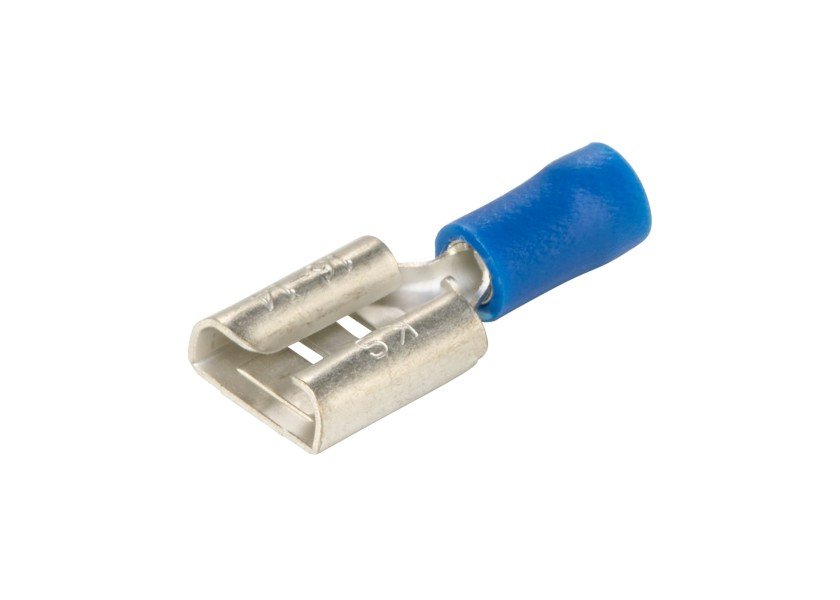
\includegraphics[width=\textwidth]{images/2-hardware/spadeConnector.png}       
        \caption{Conector de pala}
    \end{subfigure}
    \caption{Conectores utilizados en el prototipado}
    \label{fig:hardware/proto/conectores}
\end{figure}

Tanto el \texttt{LDO} como el \texttt{ESP8266} no cuentan con tornillos para su montaje, por lo que se ha realizado una placa adaptadora de baquelita. Además, se ha aprovechado para realizar las conexiones de los pines del \texttt{ESP8266} en dicha placa, facilitando la conexión con el circuito. Se pueden ver las placas en la \autoref{fig:hardware/proto/baquelitas}.

\begin{figure}[H]
    \centering
    \begin{subfigure}[b]{0.35\textwidth}
        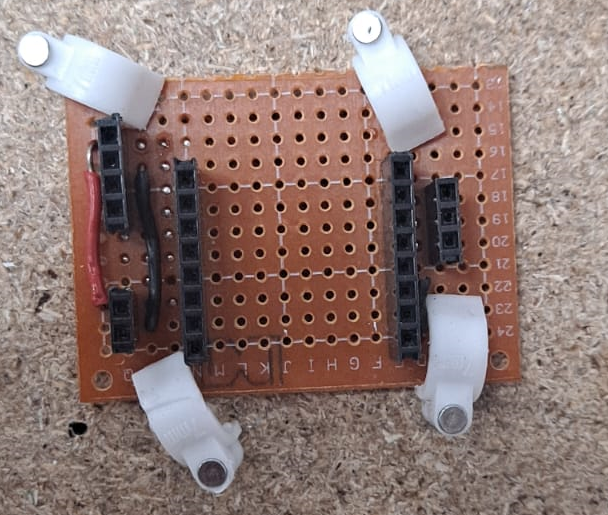
\includegraphics[width=\textwidth]{images/2-hardware/baquelitaESP.png}
        \caption{Placa para el \texttt{ESP8266}}
    \end{subfigure}
    \hspace{2cm}
    \begin{subfigure}[b]{0.35\textwidth}
        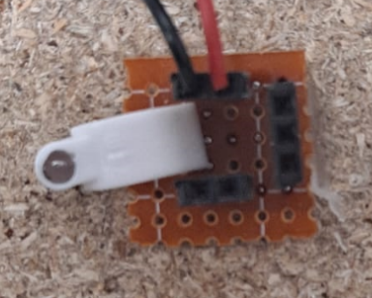
\includegraphics[width=\textwidth]{images/2-hardware/baquelitaLDO.png}
        \caption{Placa para el \texttt{LDO}}
    \end{subfigure}
    \\[0.5cm]
    \begin{subfigure}[b]{0.8\textwidth}
        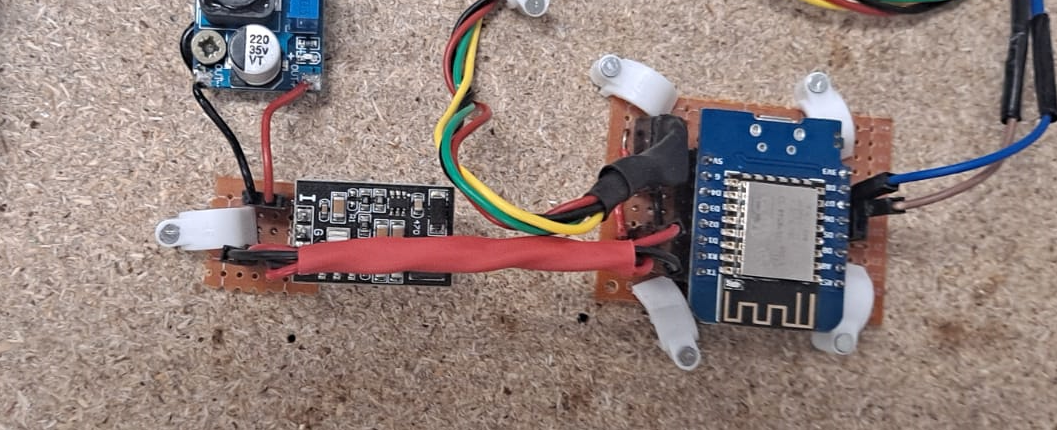
\includegraphics[width=\textwidth]{images/2-hardware/baquelitasConectadas.png}
        \caption{Placas con los módulos instalados}
    \end{subfigure}

    \caption{Placas para montaje de \texttt{LDO} y \texttt{ESP8266}}
    \label{fig:hardware/proto/baquelitas}
\end{figure}

Se puede ver el prototipo final en la \autoref{fig:hardware/proto/fotoCompleta}.

\begin{figure}[H]
    \centering
    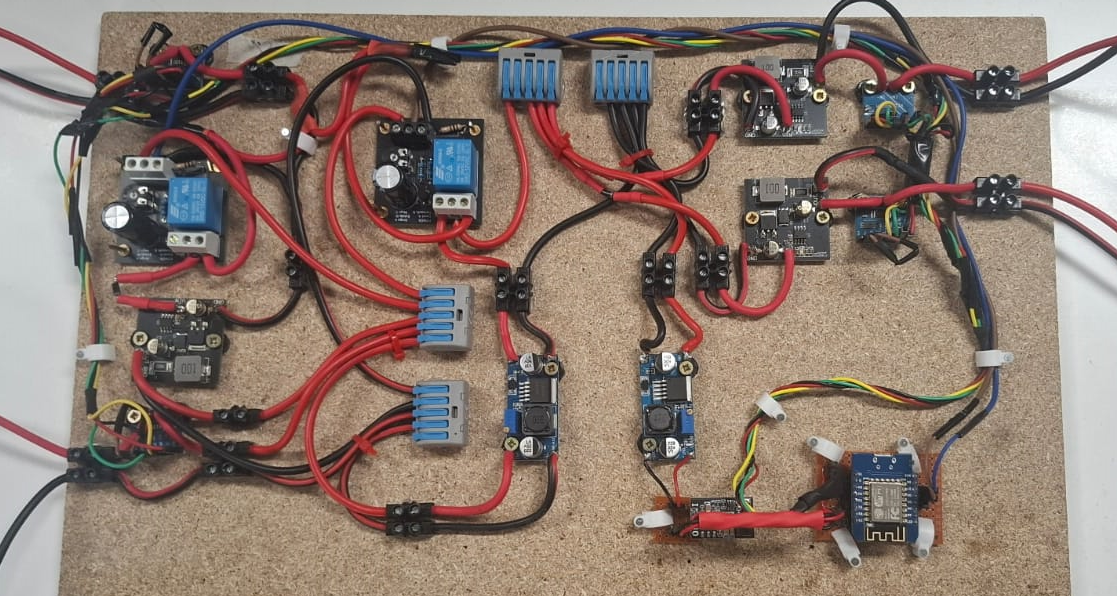
\includegraphics[width=0.9\textwidth]{images/2-hardware/circuitoFoto.png}
    \caption{Prototipo del circuito completo}
    \label{fig:hardware/proto/fotoCompleta}
\end{figure}

Con el fin de facilitar el prototipado, se utiliza la fuente de tensión del laboratorio para simular el panel solar. Cabe destacar que \textbf{la fuente no puede desconectarse por completo inmediatamente}, hay que disminuir la tensión hasta que se active la batería de \textit{Backup} y entonces se puede desactivar. Esto no es un problema en un sistema real, ya que la tensión de un panel solar no cae a $0$ inmediatamente sino que disminuye progresivamente.

Además, la batería de \textit{Backup} se puede simular con otra fuente de tensión \textbf{siempre que se desconecte la salida del cargador de dicha batería}, facilitado por el conector rápido al que está conectado.